
\documentclass[bachelor]{thesis-uestc}
\usepackage{booktabs}

\title{流媒体系统的设计与实现}
\author{}

\begin{document}

\begin{chineseabstract}

流媒体播放系统中,需要适当的传输与播放协议来实现音视频流的传输与控制,在本次课程设计中,为了尽可能优化性能和提高并发能力,选用了HLS协议作为流媒体系统核心协议。系统中服务器需要同时为多个客户提供服务,所以必须使用某种方式来支持这种多任务的服务方式。一般情况下可以有以下三种方式来选择,多进程方式、多线程方式及异步方式。在本次课程设计中,为了尽力提高服务器并发性能,采用了Epoll$+$线程池的方式进行设计。

本文介绍了m3u8索引和ts视频切片的原理与实现以及基于Epoll与线程池的服务器实现原理与方法,阐述了本次课程设计的工作内容,并给出了部分函数的定义与解释。本次课程设计实现了Linux系统下Epoll、线程池、文件缓存、HTTP响应、HLS索引生成、流视频切片的相关功能。

课程设计全部源码均已上传至GitHub:tinoryj/Server。


\chinesekeyword{C++,流媒体,视频编解码,Epoll,线程池}

\end{chineseabstract}

\thesistableofcontents

\thesischapterexordium

\section{课程设计的内容}

使用面向对象程序设计技术,采用$C++$语言,设计并实现一个功能较为复杂的流媒体系统。详细内容如下所示:

\begin{enumerate}
	\item 学习理解视频编解码等相关知识。
	\item 设计基于$HLS$协议的流媒体服务器。
	\item 设计为$HLS$协议配套的视频切片器及$m3u8$索引生成器。
	\item 利用Web浏览器作为客户端接收并播放流媒体视频文件。

\end{enumerate}


\section{课程设计的工作}

在本次课程设计中,按照模块化的思路,将epoll、线程池、http处理、文件缓存、视频切块及m3u8文件生成等模块进行了封装,以便于项目分段完成和调试。并按照软件工程设计要求完善了相关文档。

\section{报告的结构安排}
本文的章节结构安排如下:

\begin{itemize}
	\item 第一章,绪论。
 	\item 第二章,流媒体系统的需求分析报告。
	\item 第三章,系统设计中使用的相关技术的基本介绍。
	\item 第四章,流媒体系统的概要设计与分析。
	\item 第五章,流媒体系统的设计与实现。
	\item 第六章,针对流媒体系统的相关测试。
\end{itemize}

\chapter{系统需求分析}

\section{功能性需求}
\subsection{需求概述}
\subsubsection{角色定义}
在流媒体系统中,共有两种角色:

\begin{itemize}
	\item 用户:请求视频资源并观看。
	\item 系统管理员:视频预处理与服务器管理。
\end{itemize}

\subsubsection{系统功能概述}

对于用户,可以请求服务器中已经存在的视频资源并获取到该视频的编码表和数据。
对于系统管理员,可以对视频资源进行格式转化、预处理分片、查看服务器日志和管理资源。

\subsection{功能需求}

\subsubsection{功能模型}

\begin{figure}[h]
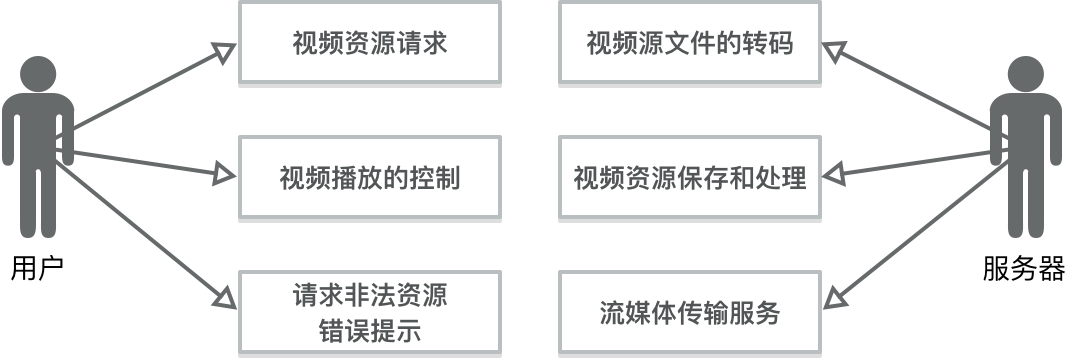
\includegraphics[width=\linewidth]{yl.png}
\caption{功能模型用例图}
\label{yl} 
\end{figure}

如上图(\ref{yl})所示为功能模型用例图,对于客户端(用户)需要提供资源请求、视频播放、播放控制、错误提示功能;对于服务器需要提供视频转码、针对传输协议的视频存储和重编码、稳定的Web响应已经系统日志功能。


\subsubsection{数据模型/对象模型}

\begin{figure}[h]
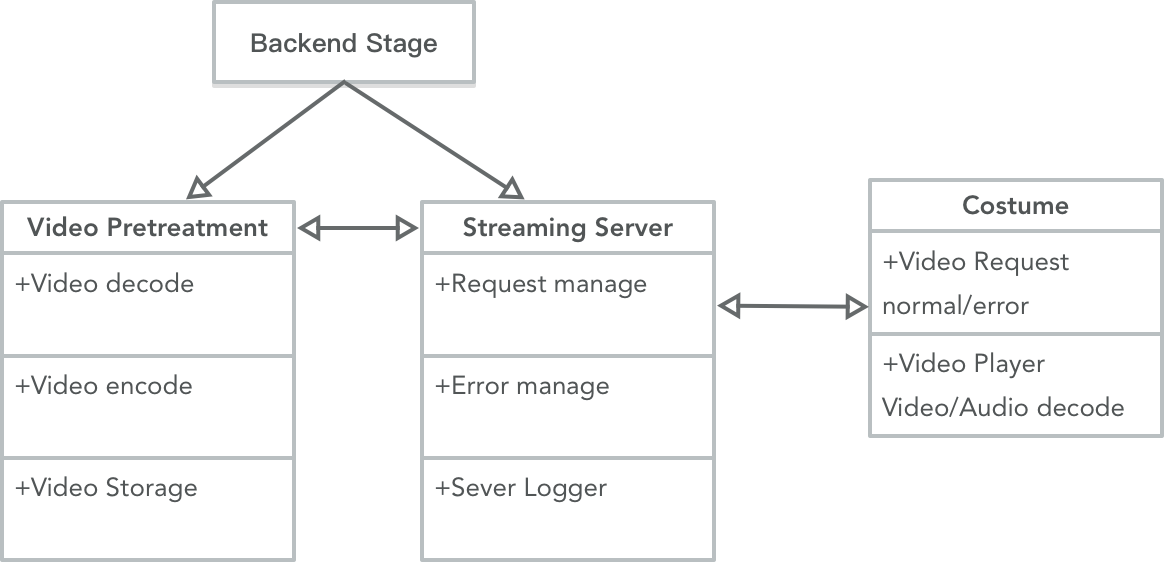
\includegraphics[width=\linewidth]{sl.png}
\caption{数据/对象模型用例图}
\label{sl} 
\end{figure}

如上图(\ref{sl})所示为数据/对象模型用例图。


\section{非功能性需求}

\begin{itemize}
	\item 对于用户请求的、确实存在的资源快速响应,保证用户视频观看体验。
	\item 服务器并发性能好,可以应对大量用户的并发访问。
	\item 对各种平台支持性能好,特别是移动平台,为用户提供优质体验。
	\item 视频预处理简单化,易于操作。
\end{itemize}

\section{本章小结}
本章主要阐述了流媒体系统的相关需求,给出了功能性和非功能性需求的具体内容,并通过用例图予以说明。

\chapter{技术基础介绍}

当前在$Internet$上传送音频和视频等信息主要有两种方式:

\begin{itemize}
	\item \textbf{下载}:完整下载一个视频,再去播放
	\item \textbf{流式传输}:如优酷、爱奇艺等视频网
\end{itemize}

在本课程设计中,使用流式传输的形式完成,常见的流媒体协议有RTP、RTCP、RTSP、MMS、HLS等,其中RTP、RTCP、RTSP一般组合使用,为了实现更高的服务器性能,本次课程设计选用了HLS协议作为传输协议。本章将给出流媒体系统所用技术的基础简介和协议选择的相关分析。

\section{流媒体播放协议}

\subsection{RTSP / RTP / RTCP协议}
三个协议需要搭配使用,才能实现流媒体播放的数据传输、控制以及稳定性保障。三个协议的详细介绍如下:

\subsubsection{RTP}


\par 实时传输协议(Real-time Transport Protocol或简写RTP)是一个网络传输协议。

\par RTP协议详细说明了在互联网上传递音频和视频的标准数据包格式。它一开始被设计为一个多播协议,但后来被用在很多单播应用中。RTP协议常用于流媒体系统(配合RTSP协议),视频会议和一键通(Push to Talk)系统(配合H.323或SIP),使它成为IP电话产业的技术基础。

\par RTP为Internet上端到端的实时传输提供时间信息和流同步,但并不保证服务质量,服务质量由RTCP来提供。RTP协议和RTCP(RTP控制协议)一起使用,而且它是创建在UDP协议上的传输层协议。

\subsubsection{RTCP}
\par 实时传输控制协议(Real-time Transport Control Protocol或RTP Control Protocol或简写RTCP)是实时传输协议(RTP)的一个姐妹协议。

\par RTCP为RTP媒体流提供信道外(out-of-band)控制。RTCP本身并不传输数据,但和RTP一起协作将多媒体数据打包和发送。RTCP定期在多媒体流会话参加者之间传输控制数据。RTCP的主要功能是为RTP所提供的服务质量(Quality of Service)提供反馈。RTCP收集相关媒体连接的统计信息,例如:传输字节数,传输分组数,丢失分组数,jitter,单向和双向网络延迟等等,网络应用程序即可利用RTCP的统计信息来控制传输的品质,比如当网络带宽高负载时限制信息流量或改用压缩比较小的编解码器。

\par 在传输层上RTP使用一个偶数UDP port;而RTCP则使用RTP的下一个port,也就是一个奇数port。

\subsubsection{RTSP}
\par 即时串流协定(Real Time Streaming Protocol,RTSP)是用来控制声音或影像的多媒体串流协议,并允许同时多个串流需求控制

\par 允许同时多个串流需求控制(Multicast),除了可以降低服务器端的网络用量,更进而支持多方视讯会议(Video Conference)。因为与HTTP1.1的运作方式相似,所以代理服务器(Proxy)的缓冲功能(Cache)也同样适用于RTSP,并因RTSP具有重新导向功能,可视实际负载情况来转换提供服务的服务器,以避免过大的负载集中于同一服务器而造成延迟。

\par 作为传输层协议,传输时所用的网络通讯协定并不在其定义的范围内,服务器端可以自行选择使用TCP或UDP来传送串流内容,它的语法和运作跟HTTP 1.1类似,但并不特别强调时间同步,所以比较能容忍网络延迟。


\subsection{RTMP / RTMPS协议}
\par RTMP(Real Time Messaging Protocol)实时消息传送协议是Adobe Systems公司为Flash播放器和服务器之间音频、视频和数据传输 开发的开放协议。它有三种变种:

\begin{itemize}
	\item 工作在TCP之上的明文协议,使用端口1935。
	\item RTMPT封装在HTTP请求之中,可穿越防火墙。
	\item RTMPS类似RTMPT,但使用的是HTTPS连接。
\end{itemize}


\par RTMP协议(Real Time Messaging Protocol)是被Flash用于对象,视频,音频的传输.这个协议建立在TCP协议或者轮询HTTP协议之上。

\par RTMP协议就像一个用来装数据包的容器,这些数据既可以是AMF格式的数据,也可以是FLV中的视/音频数据.一个单一的连接可以通过不同的通道传输多路网络流.这些通道中的包都是按照固定大小的包传输的.


\subsection{MMS (Microsoft Media Server)协议}

\par MMS(Microsoft Media Server)是一种串流媒体传送协议,用来访问并流式接收Windows Media服务器中$.asf$文件的一种协议。

\par MMS协议用于访问Windows Media发布点上的单播内容。MMS是连接Windows Media单播服务的默认方法。若观众在Windows Media Player中键入一个URL以连接内容,而不是通过超级链接访问内容,则他们必须使用MMS协议引用该流。MMS的预设埠(端口)是1755。
\par 当使用MMS协议连接到发布点时,使用协议翻转以获得最佳连接。“协议翻转”始于试图通过MMSU连接客户端。 MMSU是MMS协议结合UDP数据传送。如果MMSU连接不成功,则服务器试图使用MMST。MMST是MMS协议结合TCP数据传送。

\subsection{HLS (HTTP live streaming)协议}
\par HTTP Live Streaming(HLS)是苹果公司(Apple Inc.)实现的基于HTTP的流媒体传输协议,可实现流媒体的直播和点播,主要应用在iOS系统,为iOS设备(如iPhone、iPad)提供音视频直播和点播方案。

\par HLS点播,基本上就是常见的分段HTTP点播,不同在于,它的分段非常小。相对于常见的流媒体直播协议,例如RTMP协议、RTSP协议、MMS协议等,HLS直播最大的不同在于,直播客户端获取到的,并不是一个完整的数据流。HLS协议在服务器端将直播数据流存储为连续的、很短时长的媒体文件(MPEG-TS格式),而客户端则不断的下载并播放这些小文件,因为服务器端总是会将最新的直播数据生成新的小文件,这样客户端只要不停的按顺序播放从服务器获取到的文件,就实现了直播。

\par 由此可见,基本上可以认为,HLS是以点播的技术方式来实现直播。由于数据通过HTTP协议传输,所以完全不用考虑防火墙或者代理的问题,而且分段文件的时长很短,客户端可以很快的选择和切换码率,以适应不同带宽条件下的播放。不过HLS的这种技术特点,决定了它的延迟一般总是会高于普通的流媒体直播协议。 
 

\subsection{综述}

\par 由于MMS协议需要配和Windows Media服务器; RTMP协议需要配合Adobe Flash使用; RTP协议本身实现高并发存在极大难度,因此选择HLS协议作为流媒体系统的传输协议,在HLS协议的支持下,可以通过H5方便的在各种平台进行视频播放,同时对于火热的移动设备,使用H5可以显著降低系统资源占用电量消耗,存在较大优势。

\par 因此,本章接下来将围绕HTTP、Epoll、线程池、Cache、m3u8文件、FFmpeg、ts视频编码等方面进行介绍。

\section{TS视频编码}

ts文件为传输流文件,视频编码主要格式h264/mpeg4,音频为acc/MP3。ts文件分为三层(ts文件的三层结构如图(\ref{fig:ts})所示):

\begin{itemize}
	\item ts层(Transport Stream): 在pes层加入数据流的识别和传输必须的信息。
	\item pes层(Packet Elemental Stream): 在音视频数据上加了时间戳等对数据帧的说明信息。
	\item es层(Elementary Stream): 音视频数据。
\end{itemize}


\begin{figure}[h]
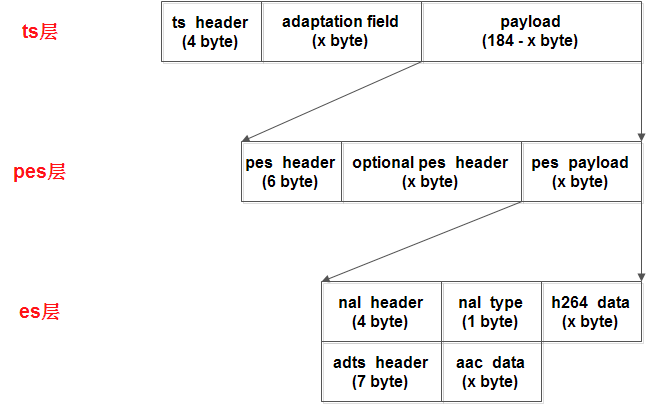
\includegraphics[width=\linewidth]{ts.png}
\caption{TS视频文件的三层结构}
\label{fig:ts} 
\end{figure}

\subsection{ts层}
ts包大小固定为188字节,ts层分为三个部分:ts header、adaptation field、 payload。ts header固定4个字节;adaptation field可能存在也可能不存在,主要作用是给不足188字节的数据做填充;payload是pes数据。

\subsubsection{TS Header}

\begin{table}[!h]
\centering
\caption{ts header各参数含义表}
\label{ts header各参数含义表}
\begin{tabular}{lp{3cm}p{6cm}p{2cm}}
\toprule
名称	&  大小 & 意义 \\
\midrule

sync\_byte	& 8b &	同步字节,固定为0x47\\
transport\_error\_indicator	& 1b &	传输错误指示符\\
payload\_unit\_start\_indicator	& 1b & 	负载单元起始标示符\\
transport\_priority	& 1b &	传输优先级,0为低优先级,1为高优先级\\
pid	& 13b &	pid值\\
transport\_scrambling\_control	& 2b &	传输加扰控制,00表示未加密\\
adaptation\_field\_control	& 2b &	是否包含自适应区,‘00’保留;‘01’为无自适应域,仅含有效负载;‘10’为仅含自适应域,无有效负载;‘11’为同时带有自适应域和有效负载。\\
continuity\_counter	& 4b & 	递增计数器,从0-f,起始值不一定取0,但必须是连续的\\
\bottomrule 
\end{tabular}
\end{table}

如上表(\ref{ts header各参数含义表})所示,为ts header的相关参数,ts层的内容是通过PID值来标识的,主要内容包括:
\begin{itemize}
	\item PAT表:指明了PMT表的PID值。
	\item PMT表:指明了音视频流的PID值。
	\item 音频流/视频流:承载音视频内容。
\end{itemize}


解析ts流要先找到PAT表,只要找到PAT就可以找到PMT,然后就可以找到音视频流了。PAT表的PID值固定为0。PAT表和PMT表需要定期插入ts流,因为用户随时可能加入ts流,这个间隔比较小,通常每隔几个视频帧就要加入PAT和PMT。PAT和PMT表是必须的,还可以加入其它表如SDT(业务描述表)等,但hls流只要有PAT和PMT就可以播放了。

\subsubsection{Adaption}

\begin{table}[!h]
\centering
\caption{Adaption域各参数含义表}
\label{Adaption域各参数含义表}
\begin{tabular}{lp{3cm}p{6cm}p{2cm}}
\toprule
名称	&  大小 & 意义 \\
\midrule

adaptation\_field\_length	& 1B	& 自适应域长度,后面的字节数\\
flag	& 1B& 	取0x50表示包含PCR或0x40表示不包含PCR\\
PCR	& 5B & 	Program Clock Reference,节目时钟参考,用于恢复出与编码端一致的系统时序时钟STC(System Time Clock)\\
stuffing\_bytes	& xB & 	填充字节,取值0xff\\
\bottomrule 
\end{tabular}
\end{table}


\par Adaption域中的各项参数如表(\ref{Adaption域各参数含义表})所示。

\par 自适应区的长度要包含传输错误指示符标识的一个字节。pcr是节目时钟参考,pcr、dts、pts都是对同一个系统时钟的采样值,pcr是递增的,因此可以将其设置为dts值,音频数据不需要pcr。如果没有字段,ipad是可以播放的,但vlc无法播放。

\par 打包ts流时PAT和PMT表是没有adaptation field的,不够的长度直接补0xff即可。视频流和音频流都需要加adaptation field,通常加在一个帧的第一个ts包和最后一个ts包里,中间的ts包不加。
     
     

\subsubsection{PAT格式}

如表(\ref{PAT表中各参数含义表}、\ref{PAT表中各参数含义表(续表)})所示为PAT表的格式信息,在进行ts文件创建时按照该格式进行编码。
\begin{table}[!h]
\centering
\caption{PAT表中各参数含义表}
\label{PAT表中各参数含义表}
\begin{tabular}{lp{3cm}p{6cm}p{2cm}}
\toprule
名称	&  大小 & 意义 \\
\midrule

table\_id	 & 8b &	PAT表固定为0x00\\
section\_syntax\_indicator	&1b&	固定为1\\
zero	&1b&	固定为0\\
reserved	&2b&	固定为11\\
section\_length	&12b&	后面数据的长度\\
transport\_stream\_id	&16b&	传输流ID,固定为0x0001\\
reserved	&2b&	固定为11\\
version\_number	&5b&	版本号,固定为00000,如果PAT有变化则版本号加1\\
current\_next\_indicator	&1b&	固定为1,表示这个PAT表可以用,如果为0则要等待下一个PAT表\\
section\_number	&8b&	固定为0x00\\
last\_section\_number	&8b&	固定为0x00\\
\bottomrule 
\end{tabular}
\end{table}

\begin{table}[!h]
\centering
\caption{PAT表中各参数含义表(续表)}
\label{PAT表中各参数含义表(续表)}
\begin{tabular}{lp{3cm}p{6cm}p{2cm}}
\toprule
名称	&  大小 & 意义 \\
\midrule
开始循环	 	\\ 
program\_number	&16b&	节目号为0x0000时表示这是NIT,节目号为0x0001时,表示这是PMT\\
reserved	&3b&	固定为111\\
PID	&13b&	节目号对应内容的PID值\\
结束循环\\	 	 
CRC32	&32b&	前面数据的CRC32校验码\\

\bottomrule 
\end{tabular}
\end{table}


\subsubsection{PMT格式}
如表(\ref{PMT表中各参数含义表}、\ref{PMT表中各参数含义表(续表)})所示为PAT表的格式信息,在进行ts文件创建时按照该格式进行编码。
\begin{table}[!h]
\centering
\caption{PMT表中各参数含义表}
\label{PMT表中各参数含义表}
\begin{tabular}{lp{3cm}p{6cm}p{2cm}}
\toprule
名称	&  大小 & 意义 \\
\midrule

table\_id	&8b&	PMT表取值随意,0x02\\
section\_syntax\_indicator	&1b&	固定为1\\
zero	&1b&	固定为0\\
reserved	&2b&	固定为11\\
section\_length	&12b&	后面数据的长度\\
program\_number	&16b&	频道号码,表示当前的PMT关联到的频道,取值0x0001\\
reserved	&2b&	固定为11\\
version\_number	&5b&	版本号,固定为00000,如果PAT有变化则版本号加1\\
current\_next\_indicator	&1b&	固定为1\\
section\_number	&8b&	固定为0x00\\
last\_section\_number	&8b&	固定为0x00\\
reserved	&3b&	固定为111\\
PCR\_PID	&13b&	PCR(节目参考时钟)所在TS分组的PID,指定为视频PID\\

reserved	&4b&	固定为1111\\
program\_info\_length	&12b&	节目描述信息,指定为0x000表示没有\\


\bottomrule 
\end{tabular}
\end{table}

\begin{table}[!h]
\centering
\caption{PMT表中各参数含义表(续表)}
\label{PMT表中各参数含义表(续表)}
\begin{tabular}{lp{3cm}p{6cm}p{2cm}}
\toprule
名称	&  大小 & 意义 \\
\midrule
开始循环	 	 \\
stream\_type	&8b&	流类型,标志是Video还是Audio还是其他数据,h.264编码对应0x1b,aac编码对应0x0f,mp3编码对应0x03\\
reserved	&3b&	固定为111\\
elementary\_PID	&13b&	与stream\_type对应的PID\\
reserved	&4b&	固定为1111\\
ES\_info\_length	&12b&	描述信息,指定为0x000表示没有\\
结束循环	 \\	 
CRC32	&32b&	前面数据的CRC32校验码\\


\bottomrule 
\end{tabular}
\end{table}



\subsection{PES层}
\par pes层是在每一个视频/音频帧上加入了时间戳等信息,pes包内容很多,以下只阐述最常用的几个参数(如表\ref{pes层主要参数含义表}所示)。

\begin{table}[!h]
\centering
\caption{pes层主要参数含义表}
\label{pes层主要参数含义表}
\begin{tabular}{lp{3cm}p{6cm}p{2cm}}
\toprule
名称	&  大小 & 意义 \\
\midrule
pes start code	& 3B &	开始码,固定为0x000001\\
stream id &	1B &	音频取值(0xc0-0xdf),通常为0xc0; 视频取值(0xe0-0xef),通常为0xe0\\
pes packet length	& 2B &	后面pes数据的长度,0表示长度不限制,
只有视频数据长度会超过0xffff\\
flag	& 1B &	通常取值0x80,表示数据不加密、无优先级、备份的数据\\
flag	& 1B &	取值0x80表示只含有pts; 取值0xc0表示含有pts和dts\\
pes data length	 &1B &	后面数据的长度,取值5或10\\
pts &	5B &	33bit值\\
dts	& 5B &	33bit值\\

\bottomrule 
\end{tabular}
\end{table}

\par pts是显示时间戳、dts是解码时间戳,视频数据两种时间戳都需要,音频数据的pts和dts相同,所以只需要pts。有pts和dts两种时间戳是B帧引起的,I帧和P帧的pts等于dts。如果一个视频没有B帧,则pts永远和dts相同。从文件中顺序读取视频帧,取出的帧顺序和dts顺序相同。dts算法比较简单,初始值+增量即可,pts计算比较复杂,需要在dts的基础上加偏移量。
\par 音频的pes中只有pts(同dts),视频的I、P帧两种时间戳均需要,视频B帧只要pts(同dts)。打包pts和dts就需要知道视频帧类型,但是通过容器格式我们是无法判断帧类型的,因此必须解析h.264内容才可以获取帧类型。
     


\subsection{ES层}
es层指的就是音视频数据,本章只介绍H.264视频和AAC音频。
\subsubsection{H.264视频}
打包h.264数据时,必须给视频数据加上一个nalu(Network Abstraction Layer unit),nalu包括nalu header和nalu type。nalu header固定为0x00000001(帧开始)或0x000001(帧中);nalu type决定了后面的H.264数据内容。H.264的数据是由slice组成的,slice的内容包括:视频、sps、pps等。nal\_unit\_type的说明如下表(\ref{nal的说明})所示。

\begin{table}[!h]
\centering
\caption{nal\_unit\_type的说明}
\label{nal的说明}
\begin{tabular}{llll}
\toprule
编码 &含义 &编码 &含义 \\
\midrule
0	&未使用 &1	&非IDR图像片,IDR指关键帧\\
2	&片分区A &3	&片分区B\\
4	&片分区C &5	&IDR图像片,即关键帧\\
6	&补充增强信息单元(SEI) &7	&SPS序列参数集\\
8	&PPS图像参数集 &9	&分解符\\
10	&序列结束 &11	&码流结束\\
12	&填充 &13$\sim$23	&保留\\
24$\sim$31	&未使用\\
\bottomrule 
\end{tabular}
\end{table}

打包es层数据时pes头和es数据之间要加入一个$type=9$的nalu,关键帧slice前必须要加入$type=7$和$type=8$的nalu,而且是紧邻(如下图(\ref{nalu})所示)。

\begin{figure}[h]
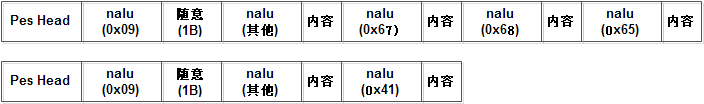
\includegraphics[width=\linewidth]{nalu.png}	
\caption{ES层数据打包格式}
\label{nalu} 
\end{figure}

\subsubsection{AAC音频}

AAC,全称Advanced Audio Coding,是一种专为声音数据设计的文件压缩格式。

\textbf{AAC音频编码的特性}

\begin{enumerate}
	\item 滤波器组(Filter bank):主要完成信号的时频转换。从而得到频域的频谱系数。
	\item 时域噪音修整(Temporal Noise Shaping,TNS):这项神奇的技术可以通过在频率域上的预测,来修整时域上的量化噪音的分布。
	\item 预测(Prediction):对音频信号进行预测可以减少重复冗余信号的处理,提高效率。
	\item 量化(Quantization):AAC的量化过程是使用两个巢状循环进行反复运算。通过对量化分析的良好控制,比特率能够被更高效地利用。
	\item 比特流格式(Bit-stream format):在AAC中,信息的传输都要经过熵编码,以保证冗余尽可能少。此外AAC拥有一个弹性的比特流结构,使得编码效率进一步提高。
	\item 长时期预测(Long Term Prediction,LTP):这是一个MPEG-4 AAC中才有的工具,它用来减少连续两个编码音框之间的信号冗余,对于处理低码率的语音非常有效。
	\item 知觉噪音代替(Perceptual Noise Substitution,PNS):这也是MPEG-4 AAC中才有的工具,当编码器发现类似噪音的信号时,并不对其进行量化,而是作个标记就忽略过去,当解码时再还原出来,这样就提高了效率。

\end{enumerate}




\section{M3U8索引}

\begin{enumerate}
	\item m3u8是一种可扩展的播放列表文件格式。它是一个包含UTF-8编码文字的m3u播放列表。m3u是包含媒体文件URL的一个事实上的播放列表标准。这种格式被用来作为HTTP Live媒体流索引文件的格式。
	\item m3u8是一种视频列表格式,里面有真正的视频的链接,另外在m3u8里面还可以再嵌套一层m3u8。
	\item m3u8是视频列表,视频编码可以是H.264等。
	\item m3u8并非苹果独占,m3u8这种列表其实编码格式是公开的。
\end{enumerate}

\subsection{M3U文件标签及属性}


\par M3U文件标签及属性说明:M3U文件中可以包含多个tag,每个tag的功能和属性如下:

\begin{itemize}
	\item \textbf{\#EXTM3U}

		每个M3U文件第一行必须是这个tag,请标示作用。
	\item \textbf{\#EXT-X-MEDIA-SEQUENCE:140651513} 

		每一个media URI 在 PlayList中只有唯一的序号,相邻之间序号+1, 一个media URI并不是必须要包含的,如果没有,默认为0
	\item \textbf{\#EXTINF:duration} 

		指定每个媒体段(ts)的持续时间(秒),仅对其后面的URI有效,title是下载资源的url
	\item \textbf{\#EXT-X-TARGETDURATION}

		指定最大的媒体段时间长(秒)。所以\#EXTINF中指定的时间长度必须小于或是等于这个最大值。这个tag在整个PlayList文件中只能出现一 次(在嵌套的情况下,一般有真正ts url的m3u8才会出现该tag)
	\item \textbf{\#EXT-X-PROGRAM-DATE-TIME}

		将一个绝对时间或是日期和一个媒体段中的第一个sample相关联,只对下一个meida URI有效,格式如\#EXT-X-PROGRAM-DATE-TIME:
	\item \textbf{\#EXT-X-ALLOW-CACHE}

		是否允许做cache,这个可以在PlayList文件中任意地方出现,并且最多出现一次,作用效果是所有的媒体段。
	\item \textbf{\#EXT-X-PLAYLIST-TYPE}

		提供关于PlayList的可变性的信息, 这个对整个PlayList文件有效,是可选的,格式如下:\#EXT-X-PLAYLIST-TYPE::如果是VOD,则服务器不能改变PlayList 文件;如果是EVENT,则服务器不能改变或是删除PlayList文件中的任何部分,但是可以向该文件中增加新的一行内容。
	\item \textbf{\#EXT-X-ENDLIST}

		表示PlayList的末尾,它可以在PlayList中任意位置出现,但是只能出现一个。
\end{itemize}


\section{HTTP协议相关内容}

\subsection{HTTP协议}

HTTP是Hyper Text Transfer Protocol(超文本传输协议)的缩写。它的发展是万维网协会(World Wide Web Consortium)和Internet工作小组IETF(Internet Engineering Task Force)合作的结果,(他们)最终发布了一系列的RFC,RFC 1945定义了HTTP/1.0版本。其中最著名的就是RFC 2616。RFC 2616定义了今天普遍使用的一个版本——HTTP 1.1。

它可以使浏览器更加高效,使网络传输减少。它不仅保证计算机正确快速地传输超文本文档,还确定传输文档中的哪一部分,以及哪部分内容首先显示(如文本先于图形)等。
\subsection{HTTP报文的格式定义}

HTTP客户程序(例如浏览器),向服务器发送请求的时候必须指明请求类型(一般是GET或者POST)。如有必要,客户程序还可以选择发送其他的请求头。大多数请求头并不是必需的,但Content-Length除外。对于POST请求来说Content-Length必须出现。 

\subsubsection{请求报文}

HTTP请求报文由请求行、请求头部、空行和请求包体4个部分组成,如图(\ref{httpreq})所示:
\begin{figure}[h]
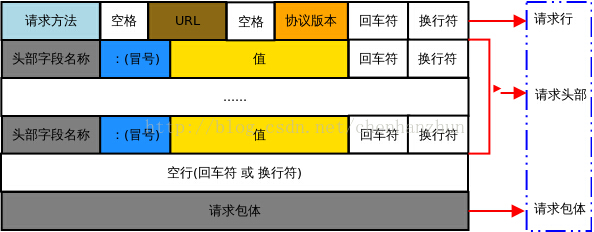
\includegraphics[width=10cm]{req.jpg}
\caption{HTTP请求报文格式}
\label{httpreq} 
\end{figure}

下面对请求报文格式进行简单的分析:

\subsubsection*{请求行}

第一行为请求行,由方法字段、URL 字段 和HTTP协议版本字段3个部分组成,他们之间使用空格隔开。常用的 HTTP 请求方法有GET、POST等。

\begin{itemize}
	\item GET:当客户端要从服务器中读取某个资源时,使用GET 方法。GET 方法要求服务器将URL 定位的资源放在响应报文的数据部分,回送给客户端,即向服务器请求某个资源。使用GET 方法时,请求参数和对应的值附加在 URL 后面,利用一个问号(“?”)代表URL 的结尾与请求参数的开始,传递参数长度受限制。
	\item POST:当客户端给服务器提供信息较多时可以使用POST 方法,POST 方法向服务器提交数据,比如完成表单数据的提交,将数据提交给服务器处理。GET 一般用于获取/查询资源信息,POST 会附带用户数据,一般用于更新资源信息。POST 方法将请求参数封装在HTTP 请求数据中,以名称/值的形式出现,可以传输大量数据。
\end{itemize}

\subsubsection*{请求头部}

请求头部由关键字/值对组成,每行一对,关键字和值用英文冒号“:”分隔。请求头部通知服务器有关于客户端请求的信息,典型的请求头有:
\begin{itemize}
	\item User-Agent:产生请求的浏览器类型。
	\item Accept:客户端可识别的响应内容类型列表;星号 “ * ” 用于按范围将类型分组,用 “ */* ” 指示可接受全部类型,用“ type/* ”指示可接受 type 类型的所有子类型。
	\item Accept-Language:客户端可接受的自然语言。
	\item Accept-Encoding:客户端可接受的编码压缩格式。
	\item Accept-Charset:可接受的应答的字符集。
	\item Host:请求的主机名,允许多个域名同处一个IP 地址,即虚拟主机。
	\item connection:连接方式(close 或 keepalive)。
	\item Cookie:存储于客户端扩展字段,向同一域名的服务端发送属于该域的cookie。
\end{itemize}

\subsubsection*{空行}


最后一个请求头之后是一个空行,发送回车符和换行符,通知服务器以下不再有请求头。

\subsubsection*{请求包体}

请求包体不在GET方法中使用,而是在POST方法中使用。POST方法适用于需要客户填写表单的场合。与请求包体相关的最常使用的是包体类型Content-Type和包体长度Content-Length。

\subsubsection{响应报文}

HTTP 响应报文由状态行、响应头部、空行和响应包体4个部分组成,如图(\ref{httpres})所示:
\begin{figure}[h]
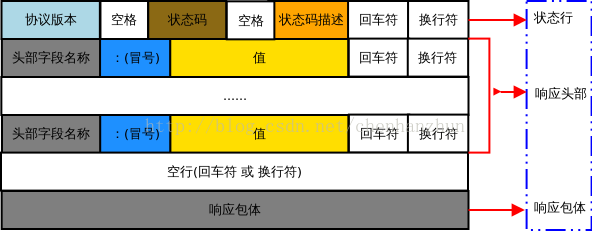
\includegraphics[width=10cm]{res.png}	
\caption{HTTP响应报文格式}
\label{httpres} 
\end{figure}

下面对响应报文格式进行简单的分析:
\subsubsection*{状态行}
状态行由HTTP协议版本字段、状态码和状态码的描述文本3个部分组成,他们之间使用空格隔开。

状态码由三位数字组成,第一位数字表示响应的类型,常用的状态码有五大类如下所示:
\begin{itemize}
	\item 1xx:表示服务器已接收了客户端请求,客户端可继续发送请求。
	\item 2xx:表示服务器已成功接收到请求并进行处理。
	\item 3xx:表示服务器要求客户端重定向。
	\item 4xx:表示客户端的请求有非法内容。
	\item 5xx:表示服务器未能正常处理客户端的请求而出现意外错误。
\end{itemize}

状态码描述文本有如下取值:

\begin{itemize}
	\item 200 OK:表示客户端请求成功。
	\item 400 Bad Request:表示客户端请求有语法错误,不能被服务器所理解。
	\item 401 Unauthonzed:表示请求未经授权,该状态代码必须与 WWW-Authenticate 报头域一起使用。
	\item 403 Forbidden:表示服务器收到请求,但是拒绝提供服务,通常会在响应正文中给出不提供服务的原因。
	\item 404 Not Found:请求的资源不存在,例如,输入了错误的URL。
	\item 500 Internal Server Error:表示服务器发生不可预期的错误,导致无法完成客户端的请求。
	\item 503 Service Unavailable:表示服务器当前不能够处理客户端的请求,在一段时间之后,服务器可能会恢复正常。
\end{itemize}

\subsubsection*{响应头部}

响应头部可包括以下信息:

\begin{itemize}
	\item Location:Location响应报头域用于重定向接受者到一个新的位置。例如:客户端所请求的页面已不存在原先的位置,为了让客户端重定向到这个页面新的位置,服务器端可以发回Location响应报头后使用重定向语句,让客户端去访问新的域名所对应的服务器上的资源。
	\item Server:Server 响应报头域包含了服务器用来处理请求的软件信息及其版本。它和 User-Agent 请求报头域是相对应的,前者发送服务器端软件的信息,后者发送客户端软件(浏览器)和操作系统的信息。
	\item Vary:指示不可缓存的请求头列表。
	\item Connection:连接方式。
	\begin{enumerate}
		\item 对于请求来说:close(告诉web服务器或者代理服务器,在完成本次请求的响应后,断开连接,不等待本次连接的后续请求);keepalive(告诉WEB服务器或者代理服务器,在完成本次请求的响应后,保持连接,等待本次连接的后续请求)。
		\item 对于响应来说:close(连接已经关闭); keepalive(连接保持着,在等待本次连接的后续请求); Keep-Alive:如果浏览器请求保持连接,则该头部表明希望web服务器保持连接多长时间(秒);例如:Keep-Alive:300。
	\end{enumerate}
\end{itemize}

\subsubsection*{空行}

最后一个响应头部之后是一个空行,发送回车符和换行符,通知服务器以下不再有响应头部。

\subsubsection*{响应包体}

服务器返回给客户端的文本信息。

\section{性能优化相关技术}


\subsection{Epoll}

epoll是Linux内核为处理大批量文件描述符而作了改进的poll,是Linux下多路复用IO接口select/poll的增强版本。

\subsubsection{Epoll的优点}
epoll可以显著提高程序在大量并发连接中只有少量活跃的情况下的系统CPU利用率。同时,在获取事件时它无须遍历整个被侦听的描述符集,只需要遍历那些被内核IO事件异步唤醒而加入Ready队列的描述符集合即可。

epoll除了提供select/poll中IO事件的水平触发(Level Triggered)外,还提供了边缘触发(Edge Triggered),使得用户空间程序有可能缓存IO状态,减少epoll\_wait/epoll\_pwait的调用,提高应用程序效率。

\begin{figure}[h]
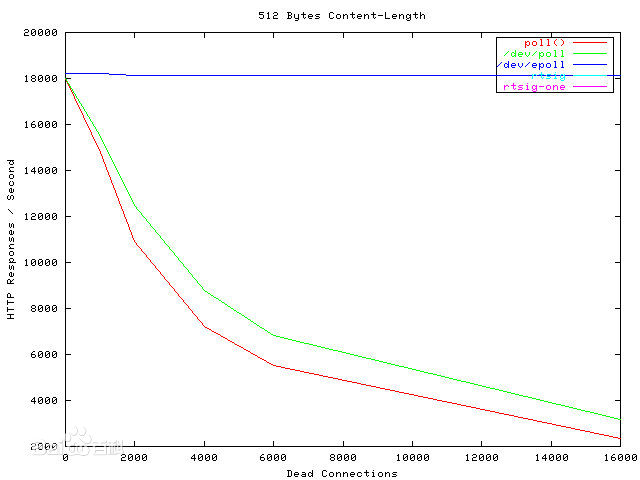
\includegraphics[width=10cm]{0.jpg}
\caption{Epoll,Poll,Select对比}
\label{0} 
\end{figure}

相对于poll和select,其主要优势有以下三点:
\begin{enumerate}
	\item 支持一个进程打开大数目的socket描述符
	\item IO效率不随FD数目增加而线性下降
	\item 使用mmap加速内核与用户空间的消息传递
\end{enumerate}


\subsubsection{Epoll的实现原理}

当服务器存在大量连接,但同时仅有少量连接处于活状态时,非常适合epoll的使用。在使用epoll实现高并发时,epoll通过在Linux内核中申请一个简易的文件系统(B+树,如图(\ref{epoll})所示)。将select/poll的调用分成了3个部分:
\begin{enumerate}
	\item 调用epoll\_create()建立一个epoll对象(在epoll文件系统中为这个句柄对象分配资源)
	\item 调用epoll\_ctl向epoll对象中添加所有连接的Socket
	\item 调用epoll\_wait收集发生的事件的连接
\end{enumerate}

\begin{figure}[h]
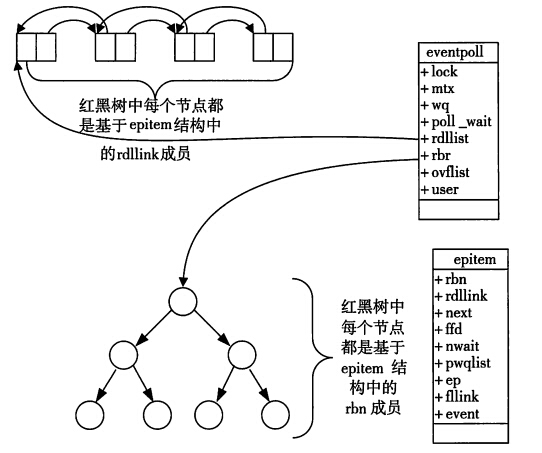
\includegraphics[width=10cm]{epoll.jpg}
\caption{Epoll数据结构示意图}
\label{epoll} 
\end{figure}

使用epoll时,只需要在进程启动时建立一个epoll对象,之后只在需要时向这个epoll对象中添加或者删除连接。

当某一进程调用epoll\_create方法时,Linux内核会创建一个eventpoll结构体,这个结构体中有两个成员与epoll的使用方式密切相关。eventpoll结构体如下所示:

\begin{lstlisting}
struct eventpoll{
    ....
    /*红黑树的根节点,这颗树中存储着所有添加到epoll中的需要监控的事件*/
    struct rb_root  rbr;
    /*双链表中则存放着将要通过epoll_wait返回给用户的满足条件的事件*/
    struct list_head rdlist;
    ....
};	
\end{lstlisting}

每一个epoll对象都有一个独立的eventpoll结构体,用于存放通过epoll\_ctl方法向epoll对象中添加进来的事件。这些事件都会挂载在红黑树中,如此,重复添加的事件就可以通过红黑树而高效的识别出来(红黑树的插入时间效率是lgn,其中n为树的高度)。

而所有添加到epoll中的事件都会与设备(网卡)驱动程序建立回调关系,也就是说,当相应的事件发生时会调用这个回调方法。这个回调方法在内核中叫ep\_poll\_callback,它会将发生的事件添加到rdlist双链表中。

在epoll中,对于每一个事件,都会建立一个epitem结构体,如下所示:

\begin{lstlisting}
struct epitem{
    struct rb_node  rbn;//红黑树节点
    struct list_head    rdllink;//双向链表节点
    struct epoll_filefd  ffd;  //事件句柄信息
    struct eventpoll *ep;    //指向其所属的eventpoll对象
    struct epoll_event event; //期待发生的事件类型
}
\end{lstlisting}
当调用epoll\_wait检查是否有事件发生时,只需要检查eventpoll对象中的rdlist双链表中是否有epitem元素即可。如果rdlist不为空,则把发生的事件复制到用户态,同时将事件数量返回给用户。

\subsubsection{Epoll的基本使用}

epoll由epoll\_create,epoll\_ctl,epoll\_wait三个基本接口组成,具体含义如下。

\textbf{epoll\_create}

在新版本的Linux内核中,epoll\_create函数的参数基本失去作用,一般调用epoll\_create(0)即可。该函数会返回一个epoll专用的文件描述符,用于操作epoll的行为\citing{fenbushi}。

\textbf{epoll\_ctl}


创建完epoll之后,使用epoll\_ctl来处理epoll中的事件,该函数原型如下所示:
\begin{lstlisting}
	int epoll_ctl(int epfd, int op, int fd, struct epoll_event *event);
\end{lstlisting}

其中第1个参数就是epoll描述符,第二个参数op表示要执行的动作,可能有3个宏。
\begin{enumerate}
	\item EPOLL\_CTL\_ADD:注册新的fd到epfd中。
	\item EPOLL\_CTL\_MOD:修改已经注册的fd中的监听事件。
	\item EPOLL\_CTL\_DEL:从epfd中删除一个fd。
\end{enumerate}

第3个参数是要监听的文件描述符,第4个参数是要监听的事件,事件的结构体定义如下所示。

\begin{lstlisting}
struct epoll_event{
	__uint32_t events;
	epoll_data_t data;
}
\end{lstlisting}

events表示事件类型,而data则是用户自定义的数据。epoll支持的事件类型如下。
\begin{enumerate}
	\item EPOLLIN:表示对应的文件描述符可读(包括对端Socket正常关闭)。
	\item EPOLLOUT:表示对应的文件描述符可写。
	\item EPOLLPRI:表示对应的文件描述符有紧急的数据可读(这里主要是有带外数据到来)。
	\item EPOLLERR:表示对应的文件描述符发生错误。
	\item EPOLLHUP:表示对应的文件描述符被挂断。
	\item EPOLLET:将epoll设置为边缘触发(Edge Triggered)模式,这是相对于水平触发(Level Triggered)来说的
	\item EPOLLONESHOT:只监听一次事件,当监听完这次事件之后,如果还需要继续监听该Socket,需要再次将这个Socket加入到epoll队列中。
\end{enumerate}

\textbf{epoll\_wait}

该函数用于等待事件发生,其原型如下所示。

\begin{lstlisting}
	int epoll_wait(int epfd, struct epoll_event *events, int maxevents, int timeout);
\end{lstlisting}

该函数的第1个参数是描述符,第2个参数是一个事件组,需要用户分配内存,第3个参数是等待的事件最大数,最后一个参数是超时事件。

\subsection{线程池与Cache}

线程池是一种多线程处理形式,处理过程中将任务添加到队列,然后在创建线程后自动启动这些任务。线程池线程都是后台线程。每个线程都使用默认的堆栈大小,以默认的优先级运行,并处于多线程单元中。如果某个线程在托管代码中空闲(如正在等待某个事件),则线程池将插入另一个辅助线程来使所有处理器保持繁忙。超过任务数最大值的线程可以排队,但他们要等到其他线程完成后才启动。

同时应用Cache将访问过的文件暂存于内存中,使得重复访问相同文件时可以避免对磁盘的I/O操作,极大的缩短处理时间,提高服务器的并发性能。

\subsubsection{使用线程池的目的}
目前的大多数网络服务器,包括Web服务器、Email服务器以及数据库服务器等都具有一个共同点,就是单位时间内必须处理数目巨大的连接请求,但处理时间却相对较短。 

传统多线程方案中我们采用的服务器模型则是一旦接受到请求之后,即创建一个新的线程,由该线程执行任务。任务执行完毕后,线程退出,这就是是“即时创建,即时销毁”的策略。尽管与创建进程相比,创建线程的时间已经大大的缩短,但是如果提交给线程的任务是执行时间较短,而且执行次数极其频繁,那么服务器将处于不停的创建线程,销毁线程的状态。

我们将传统方案中的线程执行过程分为三个过程:$T_1$、$T_2$、$T_3$。
\begin{itemize}
	\item $T_1$:线程创建时间。 
	\item $T_2$:线程执行时间,包括线程的同步等时间。 
	\item $T_3$:线程销毁时间。
\end{itemize}

那么可以看出,线程本身的开销所占的比例为$\frac{T_1+T_3}{T_1+T_2+T_3}$。如果线程执行的时间很短的话,这比开销可能占到20\%-50\%左右。如果任务执行时间很频繁的话,这笔开销将是不可忽略的。

\subsubsection{线程池的实现原理}

线程池采用预创建的技术,在应用程序启动之后,将立即创建一定数量的线程(N1),放入空闲队列中。这些线程都是处于阻塞(Suspended)状态,不消耗CPU,但占用较小的内存空间。当任务到来后,缓冲池选择一个空闲线程,把任务传入此线程中运行。当N1个线程都在处理任务后,缓冲池自动创建一定数量的新线程,用于处理更多的任务。在任务执行完毕后线程也不退出,而是继续保持在池中等待下一次的任务。如图(\ref{线程池工作方式})所示。

\begin{figure}[h]
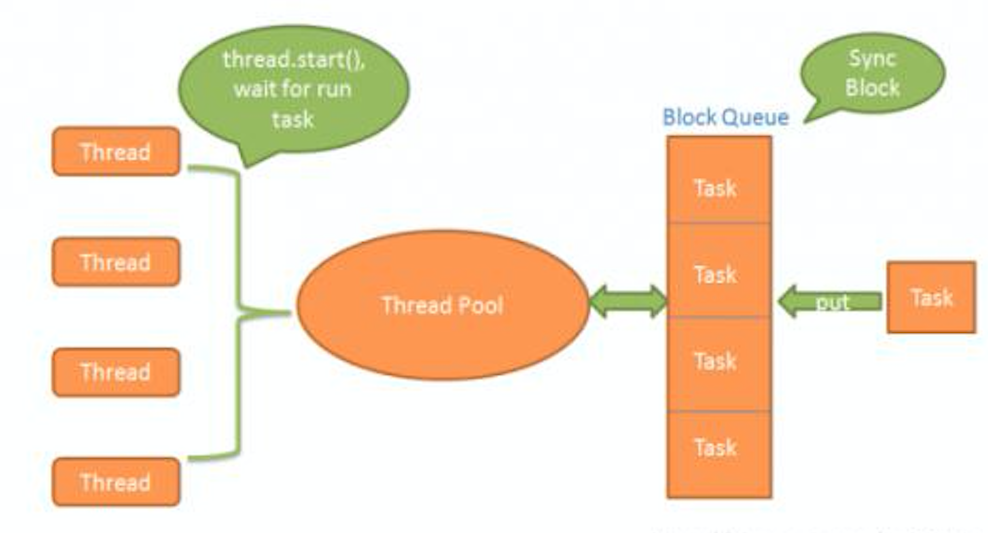
\includegraphics[width=10cm]{threadPool.png}
\caption{线程池工作方式}
\label{线程池工作方式} 
\end{figure}

同时,线程池能够减少创建的线程个数。通常线程池所允许的并发线程是有上界的,如果同时需要并发的线程数超过上界,那么一部分线程将会等待。

线程池将线程创建和销毁本身所带来的开销分摊到了各个具体的任务上,执行次数越多,每个任务所分担到的线程本身开销则越小。在这种方式下,可以极大的减小常规多线程由于线程创建、销毁带来的大量资源消耗。


\section{FFmpeg}

FFmpeg是一套可以用来记录、转换数字音频、视频,并能将其转化为流的开源计算机程序。它包括了领先的音/视频编码库libavcodec等。其包含的如下主要库将用于实现视频文件的切割分片以及m3u8文件的生成。

\begin{itemize}
	\item $libavformat$:用于各种音视频封装格式的生成和解析,包括获取解码所需信息以生成解码上下文结构和读取音视频帧等功能;
	\item $libavcodec$:用于各种类型声音/图像编解码;
	\item $libavutil$:包含一些公共的工具函数;
	\item $libswscale$:用于视频场景比例缩放、色彩映射转换;
	\item $libpostproc$:用于后期效果处理;
	\item $ffmpeg$:该项目提供的一个工具,可用于格式转换、解码或电视卡即时编码等;
	\item $ffsever$:一个 HTTP 多媒体即时广播串流服务器;
	\item $ffplay$:是一个简单的播放器,使用ffmpeg 库解析和解码,通过SDL显示;
\end{itemize}


\section{本章小结}

本章论述了流媒体传输协议的选择;HLS协议的相关内容;HTTP协议以及HTTP请求处理的基本内容;为了实现服务器高并发能力采用的Epoll、线程池、Cache等相关技术的基本概念;TS视频编码、m3u8索引的格式与建立;以及FFmpeg开源框架在视频编解码方面的相关内容。为系统的实现做好了知识和技术预备。




\chapter{系统概要设计}

根据需求分析和相关技术的选择,将流媒体系统分为了视频的预处理、Web服务器、前端播放三个主要功能模块。整个系统的工作流程如图(\ref{gysj-1})所示。首先将视频转码为流式视频文件(ts文件),然后通过切片器完成视频的预处理以生成视频分段及索引,再通过Web服务器将视频流发送至前端,最终用户通过前端H5播放器流式观看视频内容。

\begin{figure}[h]
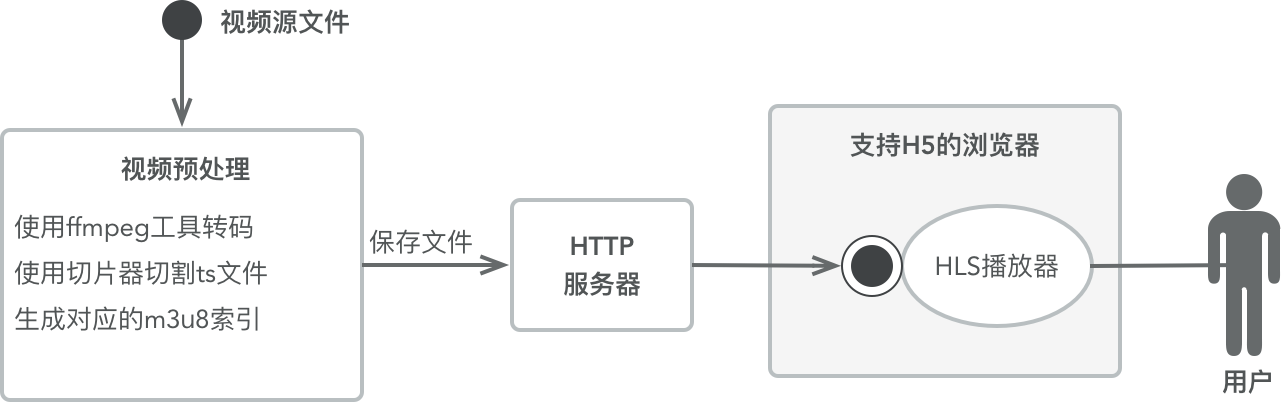
\includegraphics[width=\linewidth]{gysj-1.png}
\caption{系统工作流程}
\label{gysj-1} 
\end{figure}


\section{视频预处理}

视频的预处理分为两个主要环节:

\begin{enumerate}
	\item 将原始视频文件转码到由H.264视频编码及AAC音频编码的ts文件。
	\item 转码的到的ts文件的切块及m3u8索引的生成。
\end{enumerate}

\subsection{视频转码}

由于视频格式众多,转码需要适配的选项过多,因此使用FFmpeg工具进行转码操作,以一般mkv视频为例,可通过如下方式进行转码。

\begin{lstlisting}
	ffmpeg -i example.mkv -acodec copy -vcodec libx264 example.ts
\end{lstlisting}

同时,对于不同的原始视频文件,可以通过调整ffmpeg参数的方式实现转码。

\subsection{视频切片}

对于已经转码完成的ts视频文件,只需要按照ts文件的标准格式进行读取并重新编码即可创建出所需的ts视频分片,然后根据m3u8文件的标准格式生成对应的m3u8索引文件。

在该模块中主要通过两个方法实现:

\begin{itemize}
	\item static AVStream *add\_output\_stream
	\item int write\_index\_file
\end{itemize}

视频文件通过ffmpeg API读入之后,通过add\_output\_stream方法获取到每个视频分片的数据内容,并将数据打包写出至相应的视频分片ts文件中。 然后通过write\_index\_file方法将add\_output\_stream方法得到的每个视频分片的信息写入m3u8索引文件中。

\section{Web服务器}



\begin{figure}[h]
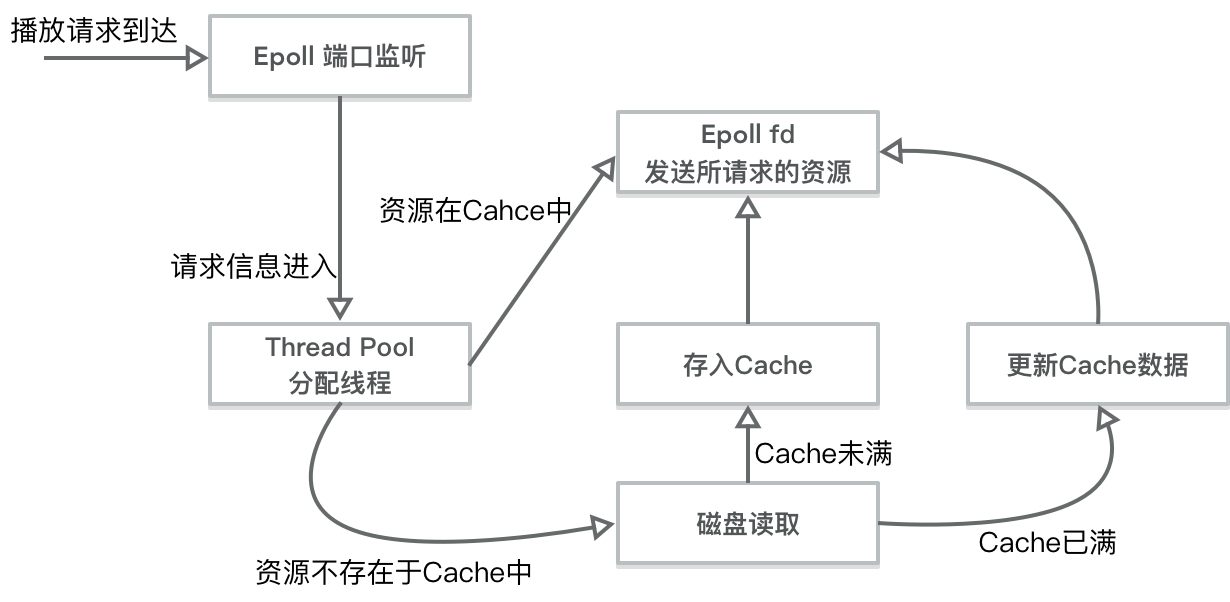
\includegraphics[width=\linewidth]{gysj-2.png}
\caption{Web服务器工作流程}
\label{gysj-2} 
\end{figure}

如上图(\ref{gysj-2})所示为Web服务器部分的工作流程图。当视频请求到达时,Epoll监听到请求并创建对应的epoll fd与之绑定,同时调用线程池中的空闲线程查询所请求的资源是否已存在于Cache中。若Cache中已存在该资源,则通过epoll fd直接从Cache中读取对应资源并发送;若Cache中不存在该资源,则响应线程发起I/O操作,从磁盘中读取该资源并检查Cache是否已满。当Cache已满时将剔除最早加入Cache的资源,并将刚读取到的资源加入Cache,当Cache未满时则直接将该资源加入Cache。最后,epoll fd发送Cache中的资源并关闭连接释放所占用的线程资源。

\section{前端播放}

对于移动端,可以通过直接请求m3u8索引文件通过H5播放基于HLS协议的流媒体文件。对于PC端,由于仅Safair浏览器支持H5的Video标签播放HLS流媒体视频文件,因此对于其他浏览器需要使用第三方的JavaScript播放框架播放视频内容。使用Video-Contrib-Hls播放框架(如下所示)实现在非移动端非Safari浏览器下的播放。


\begin{lstlisting}
<video id=example-video width=600 height=300 class="video-js vjs-default-skin" controls>
<source
     src="https://example.com/index.m3u8"
     type="application/x-mpegURL">
</video>
<script src="video.js"></script>
<script src="videojs-contrib-hls.min.js"></script>
<script>
var player = videojs('example-video');
player.play();
</script>
\end{lstlisting}


\section{本章小结}
本章主要介绍了流媒体系统的整体框架,视频预处理、web服务器和前端播放相关的概要设计,阐述了本次课程设计开发的框架与要实现的目标功能与模块。



\chapter{系统设计与实现}

\section{m3u8-segmenter的设计与实现}

在本课程设计中,定义了如下的结构体用于m3u8-segmenter的控制和调度。

\begin{lstlisting}
struct options_t {
    const char *input_file; //原始TS文件
    long segment_duration; //每个片段的时常
    const char *output_prefix; //输出片段文件的文件名前缀
    const char *m3u8_file; //输出的m3u8索引文件
    char *tmp_m3u8_file; 
    const char *url_prefix; //url前缀
    long num_segments; //总切片数目
};
\end{lstlisting}

\par 在切片程序中,通过对ffmpeg的调用,将输入的ts流视频文件分解为视频流和音频流分别处理,按照给定的分片时长分别进行切片,最终整合为分片ts文件并生成对应的m3u8索引文件。

\par 如下所示为音视频流整合输出的部分代码,通过帧率和分片时间控制,循环输出每个分片。

\begin{lstlisting}
	for (i = 0; i < ic->nb_streams && (video_index < 0 || audio_index < 0); i++) {
        switch (ic->streams[i]->codec->codec_type) {
            case AVMEDIA_TYPE_VIDEO:
                video_index = i;
                ic->streams[i]->discard = AVDISCARD_NONE;
                video_st = add_output_stream(oc, ic->streams[i]);
                break;
            case AVMEDIA_TYPE_AUDIO:
                audio_index = i;
                ic->streams[i]->discard = AVDISCARD_NONE;
                audio_st = add_output_stream(oc, ic->streams[i]);
                break;
            default:
                ic->streams[i]->discard = AVDISCARD_ALL;
                break;
        }
    }
\end{lstlisting}

如下所示为通过调用ffmpeg库实现的音视频解码和重编码的方法static AVStream *add\_output\_stream(AVFormatContext *output\_format\_context, AVStream *input\_stream)中的关键代码。
\begin{lstlisting}
	    switch (input_codec_context->codec_type) {
        case AVMEDIA_TYPE_AUDIO:
            output_codec_context->channel_layout = input_codec_context->channel_layout;
            output_codec_context->sample_rate = input_codec_context->sample_rate;
            output_codec_context->channels = input_codec_context->channels;
            output_codec_context->frame_size = input_codec_context->frame_size;
            if ((input_codec_context->block_align == 1 && input_codec_context->codec_id == CODEC_ID_MP3) || input_codec_context->codec_id == CODEC_ID_AC3) {
                output_codec_context->block_align = 0;
            }
            else {
                output_codec_context->block_align = input_codec_context->block_align;
            }
            break;
        case AVMEDIA_TYPE_VIDEO:
            output_codec_context->pix_fmt = input_codec_context->pix_fmt;
            output_codec_context->width = input_codec_context->width;
            output_codec_context->height = input_codec_context->height;
            output_codec_context->has_b_frames = input_codec_context->has_b_frames;

            if (output_format_context->oformat->flags & AVFMT_GLOBALHEADER) {
                output_codec_context->flags |= CODEC_FLAG_GLOBAL_HEADER;
            }
            break;
    default:
        break;
    }
\end{lstlisting}

由于视频分片,转码所需的时间远长于客户容忍的等待时间,因此m3u8-segmenter模块单独编译为Segmenter可执行程序,在视频放置到Web服务器中前完成切片工作,提高系统运行效率。

\section{HTTP服务器的基本设计}
在本课程设计中,定义如下5个宏,分别表示HTTP服务处于:操作成功、读、写、关闭连接以及错误状态,以便于对HTTP服务的状态进行传递与处理。
\begin{lstlisting}
#define STATUS_SUCCESS	0
#define STATUS_WRITE	1
#define STATUS_READ		2
#define STATUS_CLOSE	3
#define STATUS_ERROR	-1
\end{lstlisting}

并在HttpServe类中定义如下private变量,以完成对HTTP服务的参数设定。
\begin{lstlisting}
	static const int READ_BUFFER_SIZE = 1024; // 读缓冲区的大小
	static const int WRITE_BUFFER_SIZE = 1024; // 写缓冲区的大小
	static const char rootDir_[]; // 网页的根目录
	static const char homePage_[]; // 所指代的网页
	static Cache& cache_; // 全局cache_
	static int epollfd_;
	int sockfd_; //该HTTP连接的socket和对方的socket地址
	boost::shared_ptr<FileInfo> fileInfo_;
	char readBuf_[READ_BUFFER_SIZE]; //读缓冲区
	char postDataBuf_[READ_BUFFER_SIZE]; //请求附加内容
	size_t nRead_; //标志读缓冲区中已经读入的客户数据的最后一个字节的下一个位置
	size_t nChecked_; //当前正在分析的字符在读缓冲区中的位置
	bool keepAlive_; //是否保持连接
	bool sendFile_; //是否发送文件
	char writeBuf_[WRITE_BUFFER_SIZE]; //写缓冲区
	size_t nStored_; //写缓冲区中待发送的字节数
	size_t written_; //已经写了多少字节
\end{lstlisting}

下面是HttpServe类的定义,该类定义了HTTP服务的根目录绝对路径、文件数据读取缓存;HTTP请求到达之后的请求报文读取、uri参数的解析、所请求文件的发送、错误信息的发送方法。
\begin{lstlisting}
class HttpServe{
public:
	void init(int fd);
	void process();
	static void setEpollfd(int epollfd) {
		epollfd_ = epollfd;
	}
private:
	int processRead(); //读操作
	int processWrite(); //写操作
	void reset(); //重置
	bool addResponse(const char* format, ...); 
	bool addResponse(char *const); //
	int getLine(char *buf, int maxsize); //在请求信息缓存中读取一行
	void static getFileType(char *fileName, char *fileType); //获取文件类型信息,用于制作响应头
	void sendErrorMsg(char *cause, char *errnum, char *shortmsg, char *longmsg); //错误信息发送
	void serveStatic(char *filename, size_t fileSize); //静态网页处理
	void serveDynamic(char *text, int len); //动态网页处理
	void readRequestHdrs(); // 读取请求头
	int parseUri(char *uri, char *fileName, char *cgiargs); //处理GET路径
	bool read();
};
\end{lstlisting}

在错误信息中,实现了403、404、501三个常见错误代码的响应,并且可以动态返回错误出现原因。实现了html、css、jpg、png、otf、js、m3u8、ts等文件的发送。

\section{服务器的高性能优化}

\subsection{Epoll的设计与实现}
针对课程设计的需求,将epoll的操作封装为以下5个函数。

\begin{lstlisting}
	int setnonblocking(int fd);
	void removefd(int epollfd, int fd);
	void modfd(int epollfd, int fd, int ev);
	void addfd(int epollfd, int fd, bool one_shot);
	int Epoll_wait(int epfd, struct epoll_event* events, int maxevents, int timeout);
	int Epoll_create(int size);
\end{lstlisting}

其中Epoll\_create和Epoll\_wait函数是对原有函数epoll\_create和epoll\_wait的简单封装,以便于在发生错误时输出错误信息。setnonblocking函数用于其他函数调用,将文件描述符设置为非阻塞模式。removefd、modfd、addfd三个函数的实现如下所示。
\begin{lstlisting}
void addfd(int epollfd, int fd, bool oneShot){
	epoll_event event;
	event.data.fd = fd;
	event.events = EPOLLIN | EPOLLET; // ET触发 
	if (oneShot)
		event.events |= EPOLLONESHOT; // 设置一次性监听 
	epoll_ctl(epollfd, EPOLL_CTL_ADD, fd, &event);
	setnonblocking(fd);
}

void removefd(int epollfd, int fd){
	epoll_ctl(epollfd, EPOLL_CTL_DEL, fd, 0);
	close(fd);
}

void modfd(int epollfd, int fd, int ev){
	epoll_event event;
	event.data.fd = fd;
	event.events = ev | EPOLLET; // ET触发 
	epoll_ctl(epollfd, EPOLL_CTL_MOD, fd, &event);
}
\end{lstlisting}

addfd函数用于向epfd:epollfd中注册新的fd,第三个参数bool型oneShot用于确定是否需要将该fd设置为只监听一次事件。removefd函数封装了epoll文件描述符的删除操作,modfd用于修改已经注册过的fd的监听事件。所有要监听的事件均设置为ET触发以提高性能。

\subsection{线程池的设计与实现}
在本次课程设计中,通过参考muduo网络库,建立了一个如下所示基于生产者消费者模型的线程池类。
\begin{lstlisting}
class ThreadPool{
public:
	typedef boost::function<void()> Task; // 需要执行的任务 
	ThreadPool(int threadNum, int maxTaskNum);
	~ThreadPool(){};
	bool append(Task&&); // 往工作队列中添加任务 
	void run();
	static void* startThread(void* arg); // 任务线程 
private:
	bool isFull();
	Task take();
	size_t queueSize();
	int threadNum_; // 线程的数目
	int maxQueueSize_;
	std::list<Task> queue_; //任务队列 
	MutexLock mutex_;
	Condition notEmpty_;
	Condition notFull_;
};
\end{lstlisting}

在线程池接口处使用boost库提供的function函数代替传统的函数指针,以提供更大的灵活性,同时便于与bind函数配合使用,以取代虚函数。同时在多线程环境下,由于向缓冲区中写入数据和从缓冲区内读取数据必须互斥进行,因此引入互斥锁类(定义于mutex.hpp)完成线程的加锁、销毁操作。

如下所示,在构造函数中,包含两个条件变量用于线程调度,一个是notEmpty\_,一个是notFull\_,同时接受两个参数,一个是线程的数目,一个是最大的队列的大小。

\begin{lstlisting}
ThreadPool::ThreadPool(int threadNum, int maxQueueSize)
    : threadNum_(threadNum)
    , maxQueueSize_(maxQueueSize)
    , mutex_()
    , notEmpty_(mutex_)
    , notFull_(mutex_)
{
    assert(threadNum >= 1 && maxQueueSize >= 1);
    /* 接下来构建threadNum个线程 */
    pthread_t tid_t;
    for (int i = 0; i < threadNum; i++) {
        Pthread_create(&tid_t, NULL, startThread, this);
    }
}
\end{lstlisting}

线程池模块最重要的外部接口appand函数中,通过使用右值引用、move语义实现任务向线程池的交付。
\begin{lstlisting}
bool ThreadPool::append(Task&& task){
	{   // 使用了右值引用
		MutexLockGuard lock(mutex_); // 首先加锁
		while (isFull())
			notFull_.wait(); // 等待queue有空闲位置
		assert(!isFull());
		queue_.push_back(std::move(task)); 
		//std::cout<<"put task onto queue!"<<std::endl;
	}
	notEmpty_.notify(); // 通知任务队列中有任务可做了
}
\end{lstlisting}

在调用时只需要实例化ThreadPool类,然后调用append函数传递任务至线程池即可,具体使用如下所示。由于建立线程数目过多反而会导致性能下降,因此一般将线程池内线程数量定为处理器核心数量,以达到最佳效果。

\begin{lstlisting}
	ThreadPool pools(4, 10000); 
	pools.append(boost::bind(&HttpServe::process, &handle[sockfd]));
\end{lstlisting}

\subsection{Cache的设计与实现}

Cache类本质上就是将需要访问的文件、数据从速度较低的磁盘中预先读取到速度较快的内存中,并且建立文件名到内存地址的映射,以实现查找所需文件时快速从内存中完成,减少I/O消耗。

下面给出Cache类的定义:
\begin{lstlisting}
class FileInfo{
public:
	void *addr_; // 地址信息
	int size_; // 文件大小
	FileInfo(std::string& fileName, int fileSize); //读取文件并完成映射
	~FileInfo(); //解除映射关系
};
class Cache{
private:
	std::map<std::string, boost::shared_ptr<FileInfo>> cache_; // 实现文件名称到地址的映射
	static const size_t MAX_CACHE_SIZE = 100; // 最多缓存100个文件
	MutexLock mutex_;
public:
	Cache() : mutex_() {}
	void getFileAddr(std::string fileName, int fileSize, boost::shared_ptr<FileInfo>& ptr); //优先查找cache中是否存在指定文件,不存在时才进行读取操作(需要线程锁)
};
\end{lstlisting}


\section{本章小结}

\par 本章详细阐述了m3u8-segmenter的设计与实现;HTTP服务器端的具体设计与实现;以及针对高并发需求的Epoll、线程池、Cache等模块的相关设计。

\chapter{系统测试}

\section{视频播放测试}

使用来自电影天堂的“阳光电影www.ygdy8.com.幕后玩家.HD.720p.国语中字”作为测试用视频,原始视频文件格式为mkv。

首先通过ffmpeg转码,再使用切片器对影片完成切片(如下图(\ref{test-0})所示)。

\begin{figure}[h]
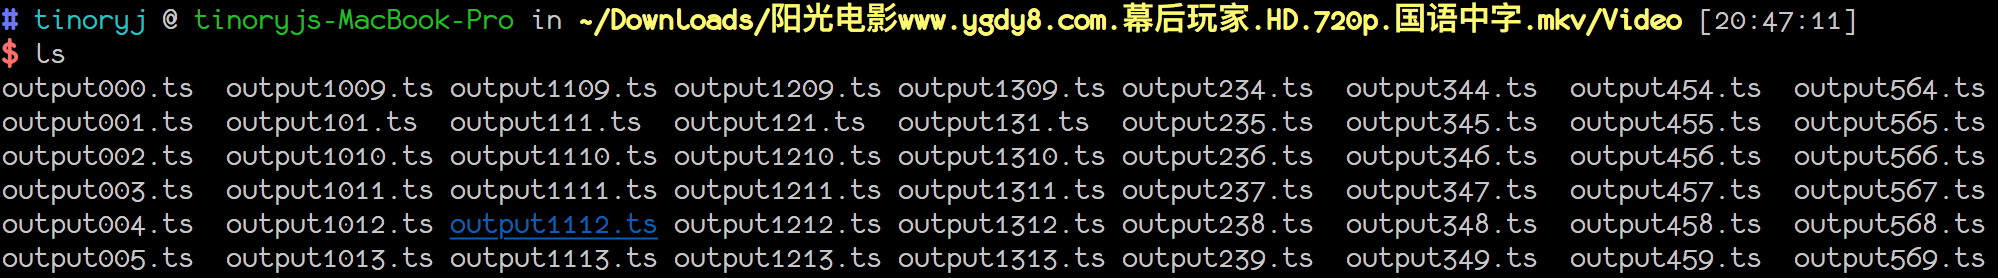
\includegraphics[width=\linewidth]{test-0.png}
\caption{视频切片结果}
\label{test-0} 
\end{figure}
生成的m3u8索引开始部分如下所示:

\begin{lstlisting}
#EXTM3U
#EXT-X-VERSION:3
#EXT-X-MEDIA-SEQUENCE:0
#EXT-X-ALLOW-CACHE:YES
#EXT-X-TARGETDURATION:14
#EXTINF:6.333333,
output000.ts
#EXTINF:10.250000,
output001.ts
#EXTINF:6.416667,
output002.ts
#EXTINF:10.416667,
output003.ts
#EXTINF:4.583333,
output004.ts
#EXTINF:2.708333,
output005.ts
#EXTINF:1.750000,
output006.ts
#EXTINF:4.500000,
output007.ts
#EXTINF:1.166667,
\end{lstlisting}

在Safari浏览器中访问0.0.0.0:8080/playlist.m3u8,可以正常观看视频,同时可以完成音量大小调节、视频播放暂停切换、进度条拖动(如下图(\ref{test-1})所示)。

\begin{figure}[h]
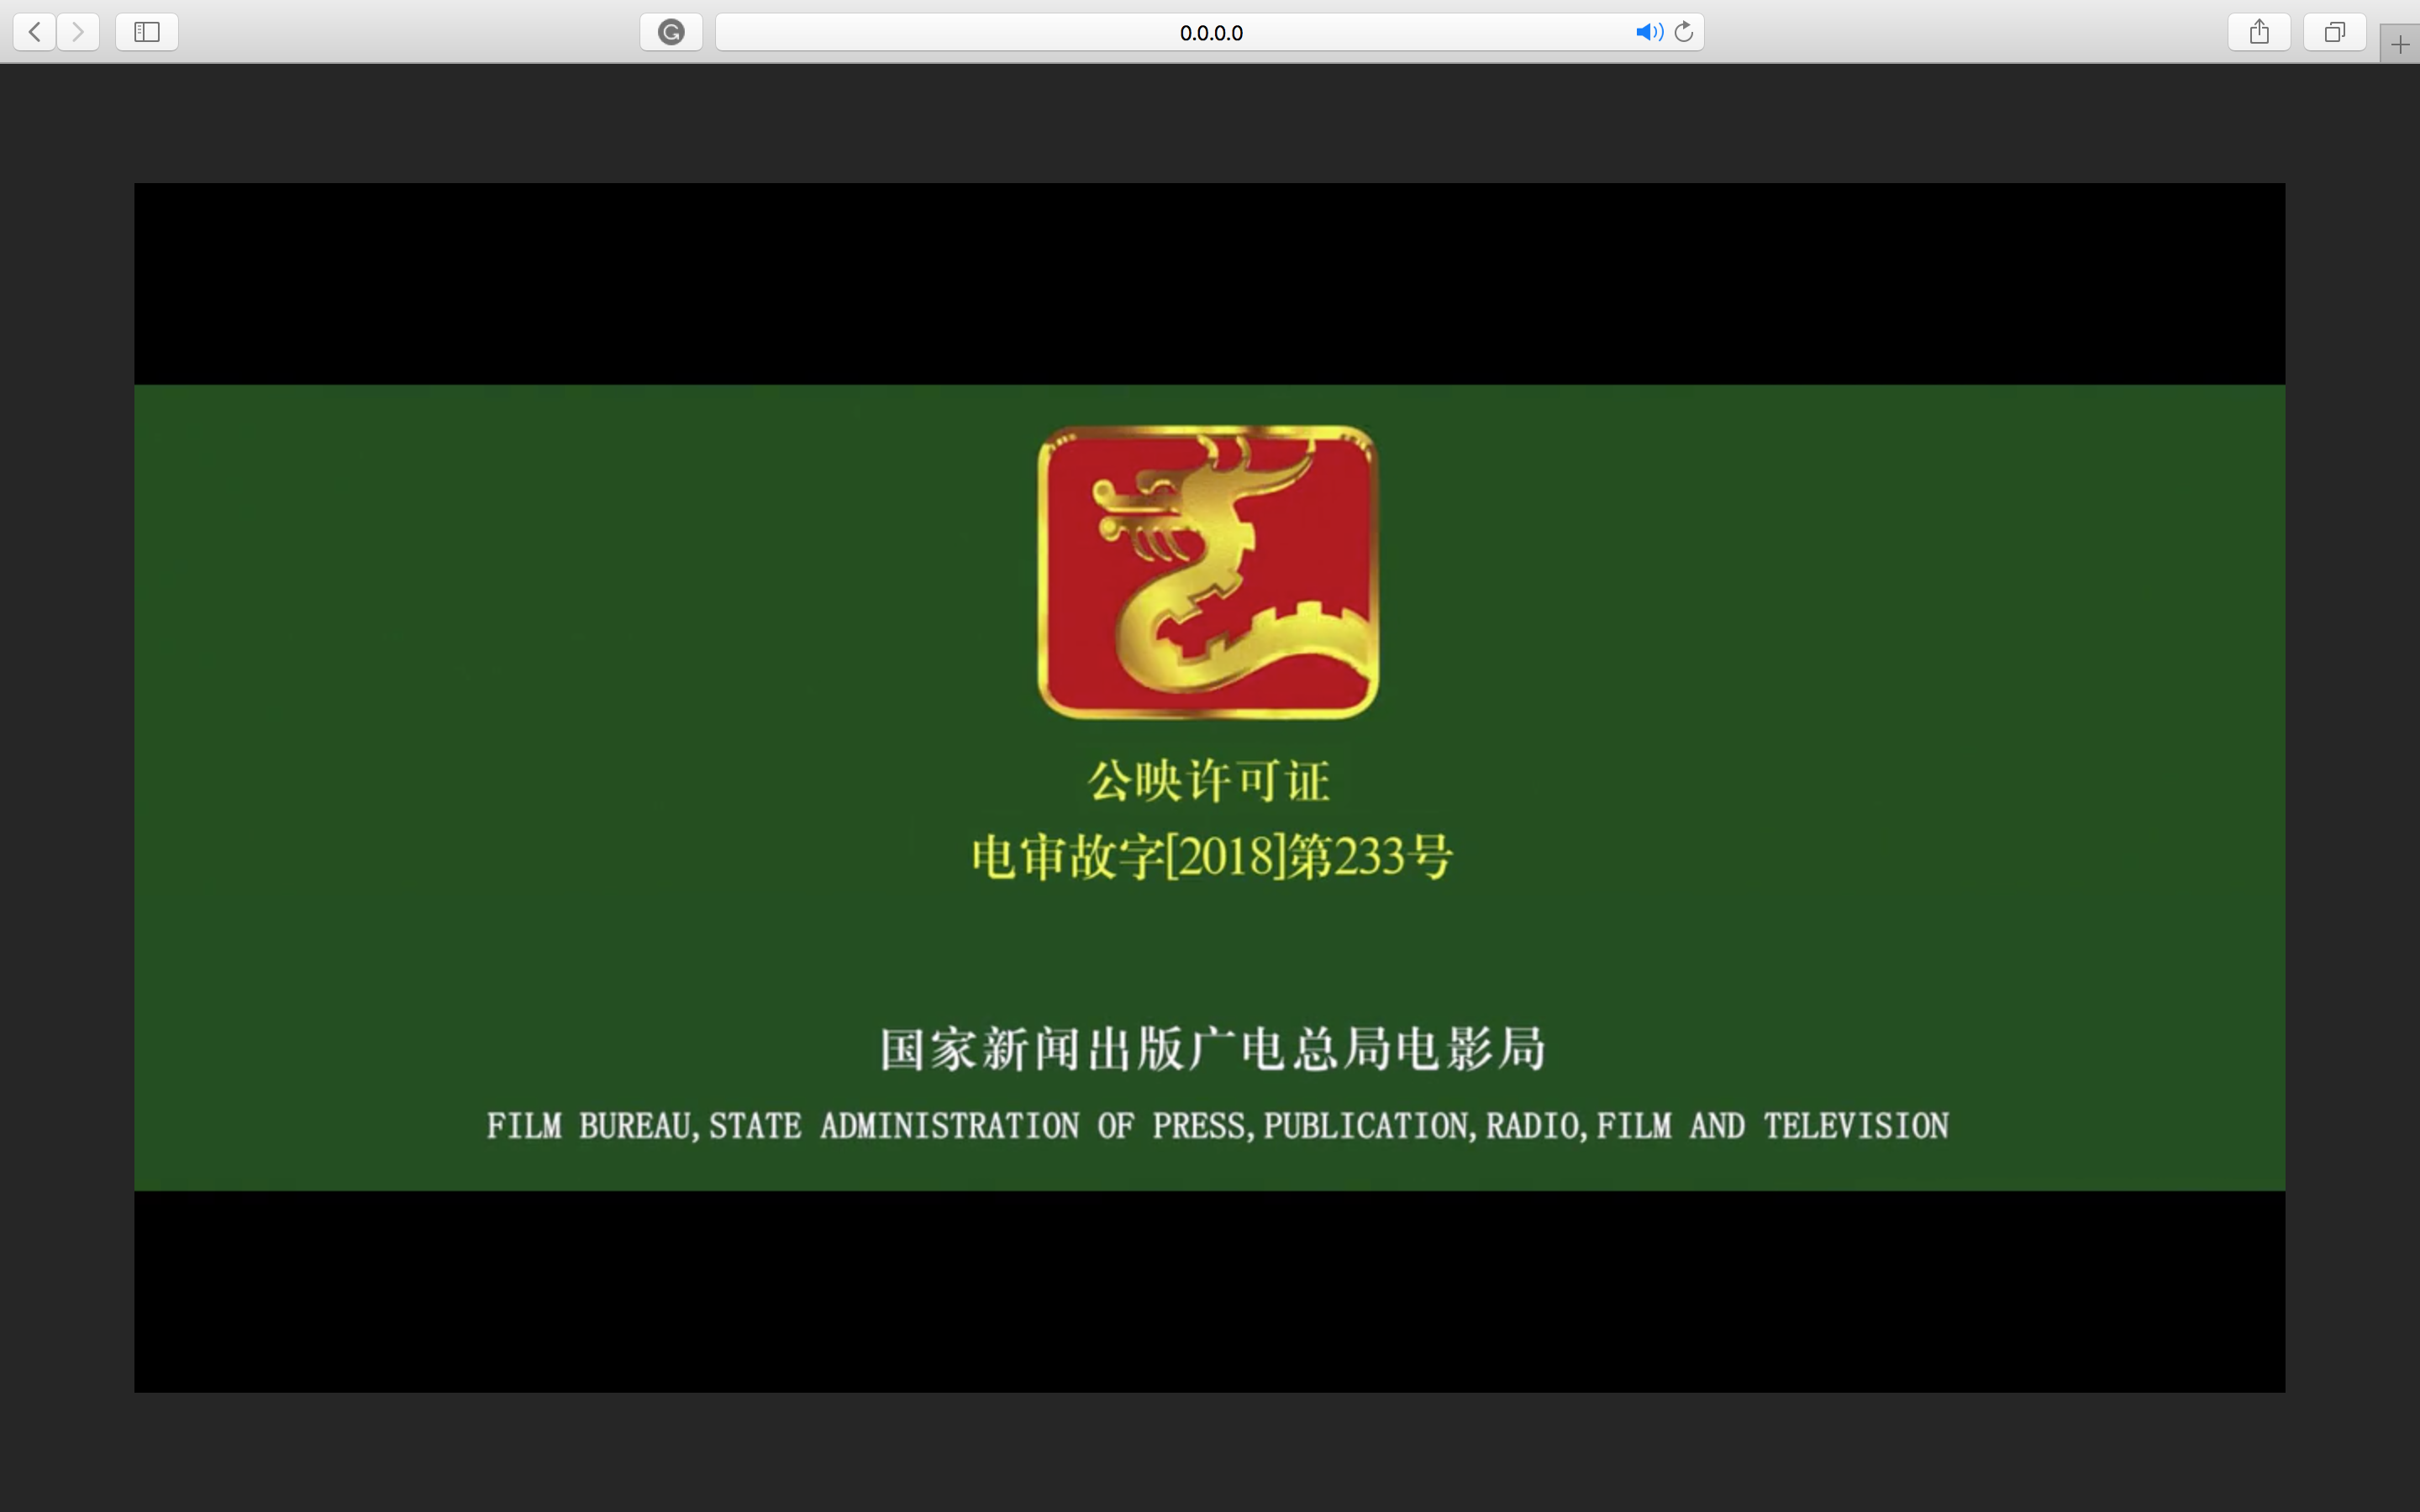
\includegraphics[width=\linewidth]{test-1.png}
\caption{视频播放测试}
\label{test-1} 
\end{figure}

\section{web服务性能测试}

本次课程设计使用webbench进行服务器性能测试。

webbench最多可以模拟3万个并发连接去测试服务器的负载能力,编译和配置简单,仅基于TCP协议上对服务器进行测试。Webbench也是开放源码,从代码上看,每个客户端都fork出一个进程进行测试,仅在TCP协议层对服务器测试,并未涉及HTTP协议。

测试环境为:

\begin{itemize}
	\item 虚拟机:VMware fusion 10.1.0
	\item CPU:Core i5 5257U (虚拟机使用一个内核两个线程)
	\item RAM:4GB
	\item 系统:Ubuntu 18.04 LTS
	\item 测试软件:webbench 1.5
\end{itemize}

测试结果如下报告所示,基本达到了预设性能目标(由于虚拟机进程fork限制,更高客户数量无法测试,因此测试结果为200个客户端测试30秒的结果)。

\begin{lstlisting}
# tinoryj @ ubuntu in ~/Desktop/webbench-1.5 [5:37:53]
$ ./webbench -c 200 http://127.0.0.1:8080/  
Webbench - Simple Web Benchmark 1.5  
Copyright (c) Radim Kolar 1997-2004, GPL Open Source Software.  
  
Benchmarking: GET http://127.0.0.1:8080/ 
200 clients, running 30 sec.  
  
Speed=246578 pages/min, 27904904 bytes/sec.  
Requests: 123079 susceed, 210 failed.  
\end{lstlisting}

\section{本章小结}

本章主要介绍了流媒体系统的使用测试以及性能测试,在使用测试部分通过两小时的影片进行了播放测试,在性能测试中使用webbench测试了服务器的并发性能与稳定能,基本达到系统设计目标。

\thesisloadbibliography[nocite]{reference}


\end{document}
